\chapter{Introduction}

This chapter introduces the importance and challenges of data integration, and provides a summary of Semantic Web technologies to demonstrate the feasibility of integrating datasets by ontology matching. The importance of instance matching is emphasised, and motivations and aims of this project are stated to formalise its research focus.


\section{Background}

% Data integration.
The ability of using data from multiple sources simultaneously has always been demanded in both research and public areas. For example, translational research data from multiple biomedical domains can be used together to track human-centered records \cite{DBLP:journals/jbi/WangLFCOHSO09}, and data exported from each peer in its own schema need to be combined in a peer-to-peer (P2P) system \cite{DBLP:conf/dbisp2p/CalvaneseDGLR03}. The process of data integration seeks to identify the semantic interconnections between information from different sources, to promote the seamlessness and effectiveness of operations across multiple datasets in such applications.
\\\\
% The semantic heterogeneity problem of data integration.
Traditional data integration has been problematic due to the semantic heterogeneity problem of datasets, which can be reflected in various aspects. Firstly, the accessibility and usability of data are unpromising, as resources are usually managed by different organisations and stored in different formats such as Excel or scanned PDF, which are not easily readable to computer programmes. In addition, without a formal representation of the semantics of knowledge within the datasets, computer programmes can only interpret the information at a very basic level \cite{DBLP:journals/expert/ShadboltBH06}, meaning that reasoning about the data can hardly be conducted. Further more, the matching process needs to be carried out even if the datasets come from the same domain of interest, due to the lack of a uniform data modelling principle and a shared vocabulary \cite{euzenat2013d}. Integration of such datasets requires huge amount of extra effort and can sometimes be unrealistic.
\\\\
% Semantic Web foundations and technologies.
The idea of Linked Data and Semantic Web provides a fundamental framework for addressing these issues. Based on the Uniform Resource Identifiers (URIs) \cite{DBLP:journals/rfc/rfc3986} and the HyperText Transfer Protocol (HTTP) \cite{DBLP:journals/rfc/rfc7540} technologies, the idea of Linked Data was formulated so that entities in the world can be uniquely identified by URIs and dereferenced with HTTP. This provides a common way to retrieve entity descriptions from the network \cite{DBLP:journals/ijswis/BizerHB09}. This framework is supplemented by the Resource Description Framework (RDF), which provides a universal, graph-based structure for the data to be modelled, and also to be queried with the SPARQL Protocol and RDF Query Language (SPARQL) \cite{DBLP:journals/tods/PerezAG09}. A shared vocabulary of a knowledge domain can be established as an ontology that is defined in the Resource Description Framework Schema (RDFS) or Web Ontology Language (OWL) \cite{DBLP:journals/expert/ShadboltBH06}, while the entires in one vocabulary can be linked to those in another with RDF triples or OWL axioms \cite{DBLP:journals/ijswis/BizerHB09}. Rules for inference purposes can be specified with the help of Rule Markup Languages (RuleML) \cite{DBLP:journals/entcs/MeiB06}.
\\\\
% Ontology matching.
With the advances of formal knowledge representation with ontologies in the context of Semantic Web, ontology matching techniques have evolved to take advantage of structured domain knowledge and assist in data integration tasks. Information coming from multiple sources are integrated without producing a newly merged dataset. Instead, they are captured by individual ontologies developed to model their respective knowledge domains, and between the ontologies, corresponding classes and instances are linked together to produce an alignment (Figure \ref{fig:align}). This alignment can be used to generate a mediator that can perform various tasks such as data translation, query reformulation and ontology merging \cite{euzenat2013d}, meaning that a query composed over a single dataset can now be reformulated as multiple queries over all the datasets, hence achieving the goal of data integration. This approach has become one of the most recognised solutions to the semantic heterogeneity problem in data integration \cite{DBLP:conf/gil/NafissiBF18}.
\\\\
\begin{figure}[ht]
\begin{center}
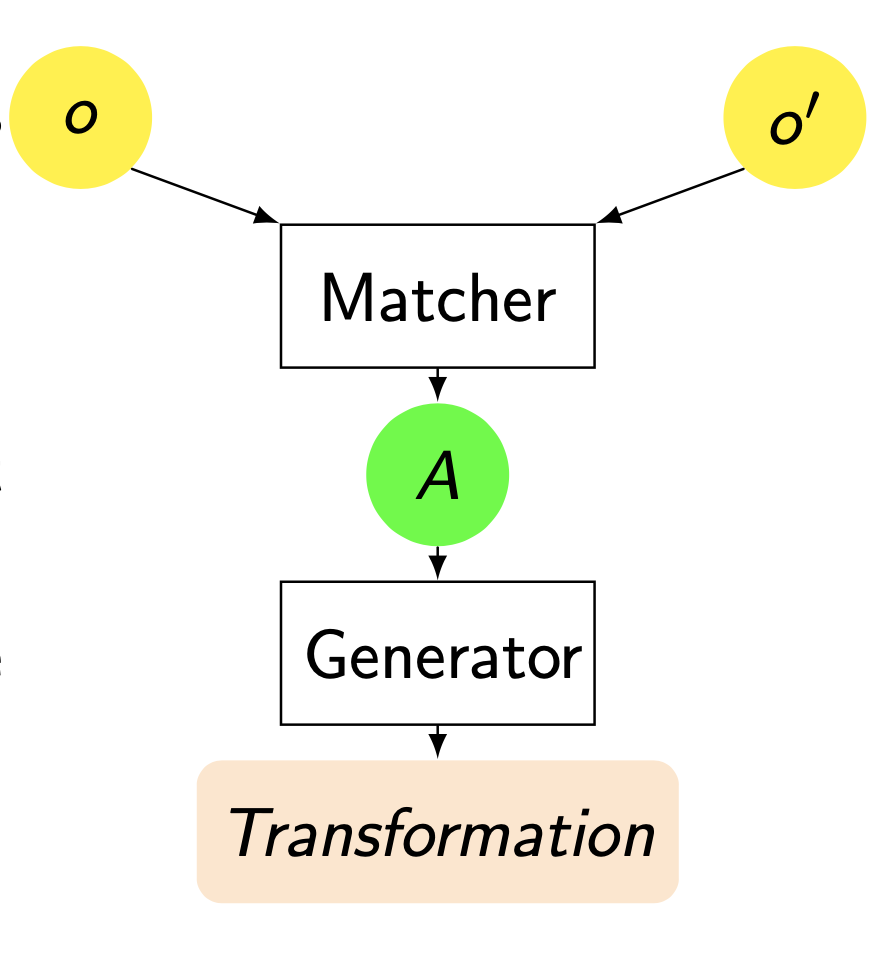
\includegraphics[width=0.3\textwidth]{img/ontomatch.png}
\caption{Alignment production}
\label{fig:align}
\end{center}
\end{figure}
\\\\
% Instance matching.
The general term ``ontology matching'' involves the matching of both terminological components (TBox), which are related to the classes or concepts, and assertional components (ABox), which are related to the instances or individuals. The concepts of TBox and ABox come from Description Logic (DL) \cite{DBLP:books/daglib/0041477}, which is the mathematical foundation of ontology languages \cite{DBLP:journals/cacm/Horrocks08}. Considering the application in data integration tasks, while the matching of TBoxes (schema-level information) is important, data are not always presented with proper schema specification \cite{DBLP:conf/boemie/CastanoFMV11}. Further more, the discovery of corresponding instances is necessary for disambiguation in the integrated dataset, and further reasoning can utilise the instance level alignment information for better performance. This has resulted in a gradual shift of research interests into the instance matching techniques in the recent years, and the introduction of such techniques have shown great achievements and potentials in popular matching systems \cite{DBLP:conf/scdm/AbubakarHMA18}.


\section{Motivation}

% Syntax and semantics of OWL and DL.
Once a dataset is formally represented by an ontology, many schema-level and instance-level information can be exploited. To demonstrate how these information can be utilised for analysis, the syntax of OWL 2 ontology entities, their corresponding representation in description logic, and their respective semantics need to be introduced. There are seven types of elementary entities in an OWL ontology\footnote{\url{https://www.w3.org/TR/owl2-syntax}}:

\begin{spacing}{1.2}
\begin{enumerate}
	\item Individual: an actual object from the knowledge domain. It can be either named or anonymous, the latter being unaccessible from outside the ontology.
	\item Class: a set of individuals governed by the same terminology.
	\item Datatype: a set of possible data values. The datatypes supported by OWL 2 are defined in the OWL 2 Datatype Map\footnote{\url{https://www.w3.org/TR/owl2-syntax/}}.
	\item Literal: a constant denoting a specific data value with the combination of a string and a datatype.
	\item Data Property: a binary relation from an individual to a literal, associating the literal as an attribute of the individual.
	\item Object Property: a binary relation from one individual to another, representing their relationship.
	\item Annotation Property: a binary relation from an entity to a comment literal, associating the annotation to the entity.
\end{enumerate}
\end{spacing}

Every entity except for literals and anonymous individuals is given an unique Internationalised Resource Identifier (IRI) \cite{DBLP:journals/rfc/rfc3987}. Examples for the elementary entities are presented in Table \ref{tab:OWL_ENTITIES} in OWL/XML syntax\footnote{\url{https://www.w3.org/2007/OWL/wiki/Primer}}.
\\

\begin{table}[h]
\resizebox{\textwidth}{!}{%
\begin{tabular}{|l|l|l|}
\hline
                     & OWL/XML Syntax                                                                                                               & Semantics                                                 \\ \hline
Individual           & \textless{}NamedIndividual IRI=``Jizhou''/\textgreater{}                                                                      & An individual called ``Jizhou''.                             \\ \hline
Class                & \textless{}Class IRI=``Student''/\textgreater{}                                                                                & A class called ``Student''.                                  \\ \hline
Datatype and Literal & \textless{}Literal datatypeIRI=``http://www.w3.org/2001/XMLSchema\#integer''\textgreater{}100\textless{}/Literal\textgreater{} & An integer literal with the value ``100''.                   \\ \hline
Data Property        & \textless{}DataProperty IRI=``hasScore''/\textgreater{}                                                                        & A potential attribute of individuals, called ``hasScore''.   \\ \hline
Object Property      & \textless{}ObjectProperty IRI=``hasSupervisor''/\textgreater{}                                                                 & A relationship between individuals called ``hasSupervisor''. \\ \hline
Annotation Property  & \textless{}AnnotationProperty IRI=``\&rdfs;comment''/\textgreater{}                                                            & An annotation that can be treated as a comment.            \\ \hline
\end{tabular}%
}
\caption{Elementary Entities in OWL 2}
\label{tab:OWL_ENTITIES}
\end{table}

Based on that, different kinds of assertions can be made between entities of an ontology. The set of assertions between classes is formally defined as TBox in description logic. Relationships between terminologies such as equivalence, inclusion and disjointness can be defined using this kind of assertions. Some examples of the TBox assertions are given in both OWL/XML syntax and description logic syntax in Table \ref{tab:OWL_DL_TBOX}.
\\

\begin{table}[h]
\resizebox{\textwidth}{!}{%
\begin{tabular}{|l|l|l|l|}
\hline
             & OWL/XML Syntax                                                                                                                                                                                                                         & Description Logic Syntax                      & Semantics                                                                                                                                                                                   \\ \hline
Equivalence  & \begin{tabular}[c]{@{}l@{}}\textless{}EquivalentClasses\textgreater\\     $\>\>\>\>$\textless{}Class IRI=``Teachers''/\textgreater\\     $\>\>\>\>$\textless{}Class IRI=``Professors''/\textgreater\\ \textless{}/EquivalentClasses\textgreater{}\end{tabular} & $\mathcal{T} \models Teachers \equiv Professors$ & \begin{tabular}[c]{@{}l@{}}The classes ``Teachers'' and ``Professors'' are equivalent in\\this ontology.\\Interpretations of ``Teachers'' and ``Professors'' are exactly\\the same set with respect to the TBox $\mathcal{T}$.\end{tabular}                  \\ \hline
Inclusion    & \begin{tabular}[c]{@{}l@{}}\textless{}SubClassOf\textgreater\\     $\>\>\>\>$\textless{}Class IRI=``Undergraduates''/\textgreater\\     $\>\>\>\>$\textless{}Class IRI=``Students''/\textgreater\\ \textless{}/SubClassOf\textgreater{}\end{tabular}           & $\mathcal{T} \models Undergraduates \sqsubseteq Students$                     & \begin{tabular}[c]{@{}l@{}}The class ``Undergraduates'' is a subclass of the class\\``Students'' in this ontology.\\Interpretation of ``Undergraduates'' is a subset of interpretation\\of ``Students'' with respect to the TBox $\mathcal{T}$.\end{tabular} \\ \hline
Disjointness & \begin{tabular}[c]{@{}l@{}}\textless{}DisjointClasses\textgreater\\     $\>\>\>\>$\textless{}Class IRI=``Boys''/\textgreater\\     $\>\>\>\>$\textless{}Class IRI=``Girls''/\textgreater\\ \textless{}/DisjointClasses\textgreater{}\end{tabular}              & $\mathcal{T} \models Boys \sqcap Girls \equiv \bot$                                  & \begin{tabular}[c]{@{}l@{}}The classes ``Boys'' and ``Girls'' are disjoint in this ontology.\\Interpretation of ``Boys'' and interpretation of ``Girls'' have\\no intersection with respect to the TBox $\mathcal{T}$.\end{tabular}                          \\ \hline
\end{tabular}%
}
\caption{TBox Assertions}
\label{tab:OWL_DL_TBOX}
\end{table}

The set of assertions involving individuals, on the other hand, is formally defined as ABox in description logic. This includes the ones that assert an individual to be an instance of a class, and the ones that specify relationships between two individuals. The latter is represented by object properties in OWL. Some examples of the ABox assertions are given in both OWL/XML syntax and description logic syntax in Table \ref{tab:OWL_DL_ABOX}.
\\

\begin{table}[h]
\resizebox{\textwidth}{!}{%
\begin{tabular}{|l|l|l|m{0.4\textwidth}|}
\hline
                          & OWL/XML Syntax                                                                                                                                                                                                                                                                                                                  & Description Logic Syntax      & Semantics                                                                                         \\ \hline
Class Assertion           & \begin{tabular}[c]{@{}l@{}}\textless{}ClassAssertion\textgreater\\ $\>\>\>\>$\textless{}Class IRI=``Student''/\textgreater\\ $\>\>\>\>$\textless{}NamedIndividual IRI=``Jizhou''/\textgreater\\ \textless{}/ClassAssertion\textgreater{}\end{tabular}                                                                                                   & $(\mathcal{T}, \mathcal{A}) \models Jizhou : Students$               & Individual ``Jizhou'' is an instance of the ``Students'' class with respect to the TBox $\mathcal{T}$ and ABox $\mathcal{A}$.                                       \\ \hline
Object Property Assertion & \begin{tabular}[c]{@{}l@{}}\textless{}ObjectPropertyAssertion\textgreater\\    $\>\>\>\>$\textless{}ObjectProperty IRI=``hasSupervisor''/\textgreater\\    $\>\>\>\>$\textless{}NamedIndividual IRI=``Jizhou''/\textgreater\\    $\>\>\>\>$\textless{}NamedIndividual IRI=``Heshan''/\textgreater\\  \textless{}/ObjectPropertyAssertion\textgreater{}\end{tabular} & $(\mathcal{T}, \mathcal{A}) \models (Jizhou, Heshan) : hasSupervisor$ & Individuals ``Jizhou'' and ``Heshan'' are bounded by the unidirectional ``hasSupervisor'' relationship with respect to the TBox $\mathcal{T}$ and ABox $\mathcal{A}$. \\ \hline
\end{tabular}%
}
\caption{ABox Assertions}
\label{tab:OWL_DL_ABOX}
\end{table}

Traditional ontology matching systems have been implemented to utilise TBox information on the schema level and ABox information on the instance level to perform reasoning activities in general. However, the expressive power of OWL 2 and description logic is far beyond that, and much more information can be made use of. Firstly, object properties in an ontology can have hierarchical and complex relationships. For example, ``hasSupervisor'' can be considered as a sub-property of ``hasTeacher'', meaning that if ``Heshan'' is a supervisor of ``Jizhou'', then ``Heshan'' must also be a teacher of ``Jizhou''. In an OWL ontology, this can be represented as:

\lstset{language=Java}
\begin{lstlisting}
    <SubObjectPropertyOf>
        <ObjectProperty IRI="hasSupervisor"/>
        <ObjectProperty IRI="hasTeacher"/>
    </SubObjectPropertyOf>
\end{lstlisting}

Other relationships between object properties include equivalence, disjointness, transitivity, reflexivity, irreflexivity, symmetry, antisymmetry and so on. They can be expressed with OWL 2 as well. In description logic, such relationships are defined as role assertions, also known as the RBox. Table \ref{tab:OWL_DL_RBOX} shows the syntax and semantics of some prominent role assertions.
\\

\begin{table}[h]
\centering
\resizebox{0.5\textwidth}{!}{%
\begin{tabular}{|l|l|}
\hline
              & Description Logic Syntax       \\ \hline
Equivalence   & $hasTeacher \equiv hasProfessor$    \\ \hline
Subsumption   & $hasSupervisor \sqsubseteq hasTeacher$   \\ \hline
Disjointness  & $Disj(isMotherOf, isFatherOf)$ \\ \hline
Transitivity  & $Trans(isAncestorOf)$          \\ \hline
Reflexivity   & $Ref(isFamilyOf)$              \\ \hline
Irreflexivity & $Irref(isParentOf)$            \\ \hline
Symmetry      & $Sym(isFriendOf)$              \\ \hline
Antisymmetry  & $Asym(isChildOf)$              \\ \hline
\end{tabular}%
}
\caption{RBox Assertions}
\label{tab:OWL_DL_RBOX}
\end{table}

In addition to that, existential and universal quantifiers can be used together with role axioms to construct complex classes. For example, the class of students doing a final year dissertation can be defined as students supervised by at least one teacher. As another example, the class of students not doing a dissertation can be defined as students who are taking only taught modules. The OWL/XML and description logic syntax for these examples are given in Table \ref{tab:OWL_DL_COMPLEX}.
\\

\begin{table}[h]
\resizebox{\textwidth}{!}{%
\begin{tabular}{|l|l|l|}
\hline
                                & OWL/XML Syntax                                                                                                                                                                                                                                                                                                                                                                                   & Description Logic Syntax                       \\ \hline
Students Doing Dissertation     & \begin{tabular}[c]{@{}l@{}}\textless{}EquivalentClasses\textgreater\\ $\>\>\>\>$\textless{}Class IRI=``StudentsDoingDT''/\textgreater\\ $\>\>\>\>$\textless{}ObjectSomeValuesFrom\textgreater\\ $\>\>\>\>\>\>\>\>$\textless{}ObjectProperty IRI=``hasSupervisor''/\textgreater\\ $\>\>\>\>\>\>\>\>$\textless{}Class IRI=``Teachers''/\textgreater\\ $\>\>\>\>$\textless{}/ObjectSomeValuesFrom\textgreater\\ \textless{}/EquivalentClasses\textgreater{}\end{tabular}    & $StudentsDoingDT \equiv \exists hasSupervisor.Teachers$      \\ \hline
Students Not Doing Dissertation & \begin{tabular}[c]{@{}l@{}}\textless{}EquivalentClasses\textgreater\\ $\>\>\>\>$\textless{}Class IRI=``StudentsNotDoingDT''/\textgreater\\ $\>\>\>\>$\textless{}ObjectAllValuesFrom\textgreater\\ $\>\>\>\>\>\>\>\>$\textless{}ObjectProperty IRI=``takeModule''/\textgreater\\ $\>\>\>\>\>\>\>\>$\textless{}Class IRI=``TaughtModules''/\textgreater\\ $\>\>\>\>$\textless{}/ObjectAllValuesFrom\textgreater\\ \textless{}/EquivalentClasses\textgreater{}\end{tabular} & $StudentsNotDoingDT \equiv \forall takeModule.TaughtModules$ \\ \hline
\end{tabular}%
}
\caption{Object Properties with Quantifiers}
\label{tab:OWL_DL_COMPLEX}
\end{table}


By combining the basic operations overs classes and the use of quantifiers with object properties, extremely complex classes can be created in an ontology. This means that the shallow structural reasoning approach adopted by most traditional ontology matching systems are less likely to discover key information hidden in those complex axioms. For example, given the following statements in description logic:
$$StudentsDoingDT \sqsubseteq Students$$
$$StudentsDoingDT \sqsubseteq \exists takeModule.DT$$
$$Students \sqsubseteq \forall takeModule.Modules$$
proper reasoning should be able to conclude that:
$$DT \sqsubseteq Modules$$
which is not obvious in any hierarchical structure. This is where description logic reasoners get superior than structural reasoning techniques. With the full capacity of handling and reasoning through such complex axioms, much more information can be extracted from ontologies and used iteratively for further reasoning. It has thus become a fundamental motivation of this project to explore the feasibility of using description logic reasoning for ontology matching.
\\\\
Apart from complex axioms, there are other insufficiently used information within the expressiveness of OWL 2 as well. To begin with, some object properties are supposed to be restricted to certain domains and ranges. As an example, the ``isSupervisorOf'' object property should be only applicable to the ``Teachers'' domain and the ``Students'' range. In an OWL ontology, this can be represented as:

\lstset{language=Java}
\begin{lstlisting}
    <ObjectPropertyDomain>
        <ObjectProperty IRI="isSupervisorOf"/>
        <Class IRI="Teachers"/>
    </ObjectPropertyDomain>
    <ObjectPropertyRange>
        <ObjectProperty IRI="isSupervisorOf"/>
        <Class IRI="Students"/>
    </ObjectPropertyRange>
\end{lstlisting}

which adds additional semantics to object properties. The structure of data properties and their respective datatypes associated with an individual are extremely useful as well. If two individuals come from equivalent classes and has very similar data properties, then it is highly probable that they are representing the same real-world object. This is another motivation of this project, to utilise such information for instance matching. Finally, since annotations can be associated with any entity in an ontology, lexical and semantic analysis can be performed on annotations to perform similarity check, instead of solely relying on the identifiers of ontology entities.


\section{Aims and Objectives}

The research focus of this project is to explore the feasibility of employing description logic reasoners for fully automated ontology matching. Algorithms have been implemented to deliver a software tool named Jonto, which was evaluated using benchmark datasets to compare with existing ontology matchers. As an ultimate aim, the produced system should be able to serve as a foundation for dataset integration. The objectives of this project are as follows:

\begin{spacing}{1.2}
\begin{enumerate}
	\item Explore and manipulate existing matching systems for ontology matching and instance matching.
	\item Design the ontology matching algorithm components, including the extraction of extra information from ontologies, the efficient representation of reasonable structures, and the reasoning steps with description logic reasoners.
    \item Implement the extraction of useful information from ontologies.
    \item Implement the data structure to efficiently index the extra information such as object properties and datatypes.
	\item Implement the discovery and repair of mappings with the help of description logic reasoners.
	\item Test and evaluate the implementation against benchmark datasets to investigate the precision, scalability and satisfiability performances of the system.
    \item If time permits, wrap the system in an official evaluation framework and add support for cross-format rendering.
\end{enumerate}
\end{spacing}

This project is interested in producing the alignment in a fully automatic manner, and tries to avoid manual parameter settings. Input ontologies are assumed to be presented in English, and are interpreted without exploiting the context-specific semantics for definitions. It should also be noted that it is not the target of the project to achieve complete correctness, which is impractical without the aid of domain expert knowledge. However, the level of precision and completeness is still considered as one of the most critical evaluation criterion. The underlying reasonability and decidability of the logic will also be taken into account.


\section{Report Outline}

This chapter has summarised the general background of Semantic Web technologies and the motivation of reasoning based ontology matching for data integration. Chapter 2 provides a detailed description of previous works related to ontology matching, and mentions the most prominent matching systems at the present. Chapter 3 explains the methodologies used in the design of the system structure and related algorithms. Chapter 4 then demonstrates the details of implementation, illustrating the algorithms with code fragments and introducing the tools and frameworks used. Chapter 5 shows the evaluation results according to ontologies with different characteristics, and does a comparison between the proposed ontology matching system and other major systems. Finally, chapter 6 presents the project management and reflections along the progress.
